\documentclass[11pt,a4paper]{article}

% ====== PAQUETES ======
\usepackage[spanish]{babel}
\usepackage[T1]{fontenc}
\usepackage{libertinus}
\usepackage{tikz}
\usepackage{graphicx}
\usepackage{geometry}
\usepackage{tabularx}
\usepackage{booktabs}
\usepackage{xcolor}
\usepackage{fancyhdr}
\usepackage{titlesec}
\usepackage{chngcntr}
\usepackage{caption}
\usepackage{url}    
\usepackage{hyperref}
\usepackage{float}
\usepackage[cache=false]{minted}
\usepackage{pifont}
\usepackage{hyperref}
\newcommand{\cmark}{\ding{51}}

% ====== MÁRGENES ======
\geometry{top=2.5cm, bottom=3cm, left=2.5cm, right=2.5cm}
\setlength{\parindent}{0pt}

% ====== COLORES ======
\definecolor{azulceu}{RGB}{0,70,140}
\colorlet{azulceu}{azulceu!80!white}
\definecolor{grisclaro}{gray}{0.3}
\definecolor{codegray}{gray}{0.95}
\definecolor{linkblue}{RGB}{0, 102, 204}
\hypersetup{
    colorlinks=true,
    linkcolor=linkblue,
    urlcolor=linkblue,
    citecolor=linkblue
}

% ====== ENCABEZADO ======
\pagestyle{fancy}
\fancyhf{}
\fancyhead[L]{\small\textsc{Ingeniería Matemática\\Aprendizaje Automático}}
\fancyhead[R]{
\includegraphics[scale=0.13]{img/ceu.png}}
\fancyfoot[C]{\thepage}
\setlength{\headheight}{29.52pt}

% ====== TÍTULOS ======
\titleformat{\section}{\Large\bfseries\color{azulceu}}{\thesection}{1em}{}
\titleformat{\subsection}{\large\bfseries\color{grisclaro}}{\thesubsection}{1em}{}

% ====== INICIO DEL DOCUMENTO ======
\begin{document}
\begin{titlepage}
\begin{tikzpicture}[remember picture, overlay]

  % Fondo general gris claro
  \fill[codegray] (current page.south west) rectangle (current page.north east);

  % Franja vertical azul a la izquierda
  \fill[azulceu] (current page.south west) rectangle ([xshift=6cm]current page.north west);

  % Logo en la parte superior izquierda
  \node[anchor=north west, xshift=0cm, yshift=-1.2cm] at (current page.north west)
    {
\includegraphics[width=6cm]{img/ceubw.png}};

  % Título dentro de la franja azul
  \node[align=center, text=white, font=\bfseries\Huge] at ([xshift=3cm, yshift=-7cm]current page.north west)
    {MEMORIA\\PROYECTO};

  % Título principal elegante
  \node[align=center, text=azulceu, font=\bfseries\fontsize{20pt}{24pt}\selectfont] 
    at ([xshift=13.5cm, yshift=-15cm]current page.north west)
    {Aprendizaje Automático:\\[0.7em] \textsc{Predicción del Rendimiento Académico}};

  % Universidad
  \node[align=left, text=black, font=\bfseries\large] at ([xshift=13.5cm, yshift=10.5cm]current page.south west)
    {Universidad CEU San Pablo};

  % Autores del trabajo
  \node[align=center, text=black, font=\Large\itshape] at ([xshift=13.5cm, yshift=6.8cm]current page.south west)
    {David Ruiz Luque\\Alberto García Caballero\\Ricardo Marín Fernández-Conde};

  % Fecha centrada
  \node[align=center, text=black, font=\normalsize] at ([xshift=13.5cm, yshift=2.8cm]current page.south west)
    {15 de abril de 2025};

\end{tikzpicture}
\end{titlepage}


% ====== ÍNDICE ======
\newpage
\large
\tableofcontents
\thispagestyle{empty}
\newpage
\normalsize

% ====== REINICIAR NUMERACIÓN ======
\cleardoublepage
\pagenumbering{arabic}
\setcounter{page}{1}
\fancyfoot[C]{\raisebox{-10pt}{\thepage}}


% ====== INTRODUCCIÓN ======
\section{Introducción}

El aprendizaje automático es una disciplina fundamental dentro de la inteligencia artificial que permite a las máquinas aprender a partir de datos y tomar decisiones sin haber sido programadas explícitamente para cada tarea. En este proyecto, hemos aplicado diversas técnicas de aprendizaje automático con el objetivo de desarrollar un modelo capaz de predecir el rendimiento académico de estudiantes a partir de datos reales.

\medskip

La motivación detrás de este trabajo radica en la relevancia del rendimiento educativo como factor determinante en la trayectoria personal y profesional de los individuos. Comprender qué variables influyen en el desempeño académico puede ser de gran utilidad para instituciones educativas, docentes y responsables de políticas públicas.

\medskip

El proyecto se ha desarrollado utilizando el conjunto de datos \textbf{Student Performance Data Set}, obtenido del \textit{UCI Machine Learning Repository}, una fuente de referencia en el ámbito académico. La información del dataset está disponible en el siguiente \href{https://archive.ics.uci.edu/ml/datasets/student+performance}{\textcolor{linkblue}{enlace}}. 

\medskip

El análisis realizado incluye tareas esenciales como la limpieza y preprocesamiento de datos, análisis estadístico, exploración visual, ingeniería de características y, finalmente, la construcción y validación de distintos modelos predictivos. Además, se ha llevado a cabo una comparación entre los modelos propuestos teniendo en cuenta criterios de precisión, interpretabilidad, coste computacional e interés práctico.

\medskip

En las siguientes secciones se describen de manera detallada todas las fases del proyecto, incluyendo la descripción del conjunto de datos, la metodología seguida, los resultados obtenidos y las conclusiones derivadas del trabajo realizado.

\section{Metodología y objetivos}

En este proyecto se aborda un problema de aprendizaje automático en el ámbito educativo: \textbf{predecir la expectativa académica del alumnado} a partir de variables contextuales, personales y de rendimiento académico previo.

El objetivo principal es \textbf{construir un modelo predictivo que permita anticipar la expectativa académica (\texttt{esp})} de cada estudiante. Este enfoque tiene un impacto práctico relevante, ya que puede ayudar a:
\begin{itemize}
  \item Identificar estudiantes en riesgo de bajo rendimiento.
  \item Apoyar a docentes y orientadores con herramientas de diagnóstico.
  \item Diseñar estrategias educativas más personalizadas.
\end{itemize}

Para alcanzar este objetivo, se han seguido todas las etapas del ciclo completo de un proyecto de aprendizaje automático:
\begin{enumerate}
  \item Preparación y limpieza del conjunto de datos.
  \item Análisis exploratorio y estadístico.
  \item Ingeniería de atributos relevantes.
  \item Entrenamiento y evaluación de diversos modelos de clasificación.
  \item Aplicación de técnicas de mejora (balanceo de clases, ajuste de hiperparámetros).
  \item Evaluación integral del modelo final (precisión, interpretabilidad y coste computacional).
\end{enumerate}

Esta metodología garantiza un enfoque riguroso y reproducible, permitiendo obtener conclusiones sólidas sobre la capacidad predictiva de los modelos aplicados y su utilidad en el contexto educativo.

% ====== DESCRIPCIÓN DEL CONJUNTO DE DATOS ======
\section{Descripción del conjunto de datos}

Nuestro dataset contiene información académica, demográfica y socioeconómica de estudiantes indios de nivel preuniversitario. El objetivo principal del análisis es predecir el nivel de rendimiento académico de cada estudiante, clasificado en categorías como \textit{Good}, \textit{Average} y \textit{Poor}, a partir de sus características personales y familiares.

\medskip

El conjunto de datos cuenta con \textbf{131 instancias} y \textbf{22 atributos}, todos ellos de tipo categórico. A continuación, se analiza brevemente cada una de las variables:

\begin{table}[H]
\centering
\footnotesize
\renewcommand{\arraystretch}{1.1}
\begin{tabularx}{\textwidth}{|l|X|X|}
\hline
\textbf{Var.} & \textbf{Descripción} & \textbf{Influencia en \texttt{atd}} \\
\hline
\texttt{ge} & Género (M/F) & Diferencias culturales/contextuales \\
\texttt{cst} & Casta/grupo social & Relación con nivel socioeconómico \\
\texttt{tnp} & Nota 1er parcial & Indicador de rendimiento \\
\texttt{twp} & Nota 2º parcial & Refuerza patrón de rendimiento \\
\texttt{iap} & Evaluación interna & Influencia directa en resultado \\
\texttt{esp} & Participación/exposición & Evalúa habilidades comunicativas \\
\texttt{arr} & ¿Alojamiento? (Y/N) & Afecta entorno y tiempo de estudio \\
\texttt{ms} & Estado civil & Poco relevante (mayoría solteros) \\
\texttt{ls} & Medio transporte (T/V) & Influye en cansancio/dedicación \\
\texttt{as} & Tipo admisión & Refleja situación económica \\
\texttt{fmi} & Ingreso familiar & Recursos académicos disponibles \\
\texttt{fs} & Tamaño familia & Carga y apoyo familiar \\
\texttt{fq} & Educación padre & Entorno educativo en casa \\
\texttt{mq} & Educación madre & Igual de relevante que paterna \\
\texttt{fo} & Ocupación padre & Nivel económico indirecto \\
\texttt{mo} & Ocupación madre & Complementa perfil socioeconómico \\
\texttt{nf} & Nº miembros familia & Recursos/atención diluidos \\
\texttt{sh} & Salud general & Relacionado con rendimiento \\
\texttt{ss} & Tipo escuela previa & Nivel de preparación previa \\
\texttt{me} & Idioma instrucción & Comprensión si no es nativo \\
\texttt{tt} & Tiempo transporte & Menos tiempo de estudio \\
\texttt{atd} & \textit{Objetivo}: rendimiento final & Etiqueta a predecir \\
\hline
\end{tabularx}
\caption*{Descripción resumida de las variables}
\end{table}

\medskip

Seguidmente, se muestra un extracto de las primeras cinco filas del conjunto de datos:

\begin{minted}[fontsize=\small, bgcolor=codegray]{python}
from scipy.io import arff
import pandas as pd

# Cargar el archivo ARFF
data, meta = arff.loadarff('Sapfile1.arff')
df = pd.DataFrame(data)

# Mostrar las primeras filas del dataset para revisión inicial
df.head()
\end{minted}

\begin{table}[H]
\centering
\footnotesize
\begin{tabular}{lllllllllll}
\textbf{ge} & \textbf{cst} & \textbf{tnp} & \textbf{twp} & \textbf{iap} & \textbf{esp} & \textbf{arr} & \textbf{ms} & \textbf{ls} & \textbf{as} & \textbf{...} \\
F & G & Good & Good & Vg & Good & Y & Unmarried & V & Paid & ... \\
M & OBC & Vg & Vg & Vg & Vg & N & Unmarried & V & Paid & ... \\
F & OBC & Good & Good & Vg & Good & N & Unmarried & V & Paid & ... \\
M & MOBC & Pass & Good & Vg & Good & N & Unmarried & V & Paid & ... \\
M & G & Good & Good & Vg & Vg & N & Unmarried & V & Paid & ... \\
\end{tabular}
\caption*{Primeras filas del conjunto de datos}
\end{table}

\medskip

Este conjunto de datos permite explorar cómo distintas dimensiones personales y familiares pueden influir en el rendimiento escolar, ofreciendo una oportunidad interesante para aplicar técnicas de aprendizaje automático supervisado.

\section{Preprocesamiento de datos}

El preprocesamiento es una etapa clave en todo flujo de trabajo de aprendizaje automático. En este proyecto, se han realizado varias operaciones fundamentales antes de entrenar los modelos. A continuación, se detallan los pasos realizados:

\subsection{Conversión de valores byte a string}

El conjunto de datos, al estar en formato \texttt{.arff}, contenía sus valores almacenados como secuencias de bytes (e.g., \texttt{b'Good'}). Para poder analizarlos con herramientas como \texttt{pandas}, se realizó una conversión de todos estos valores a cadenas de texto (\texttt{str}) mediante una transformación a nivel de celda.

\medskip

\subsection{Verificación de valores nulos}

Se comprobó si alguna de las 22 columnas contenía valores nulos. La inspección mostró que \textbf{no hay valores faltantes} en ninguna de las variables, lo cual facilitó el flujo de trabajo al no ser necesaria ninguna imputación ni eliminación de observaciones.

\begin{minted}[bgcolor=codegray]{text}
Valores nulos por columna:
ge     0
cst    0
...
atd    0
\end{minted}

\medskip

\subsection{Clasificación de variables por tipo}

Se identificaron las variables categóricas y numéricas mediante la inspección del tipo de dato de cada columna:

\begin{itemize}
  \item Todas las variables del conjunto fueron clasificadas como categóricas (\texttt{object}).
  \item No se identificaron variables numéricas.
\end{itemize}

\medskip

\subsection{Análisis descriptivo de variables categóricas}

Se utilizaron las funciones estadísticas de \texttt{pandas} para obtener una visión general de cada variable categórica. Para cada una se reportaron:

\begin{itemize}
  \item \textbf{count}: número total de observaciones.
  \item \textbf{unique}: número de valores únicos presentes.
  \item \textbf{top}: valor más frecuente.
  \item \textbf{freq}: frecuencia de ese valor más frecuente.
\end{itemize}

\begin{minted}[bgcolor=codegray]{text}
Estadísticas para variables categóricas:
ge:     2 categorías (M, F), valor más común: M (72 casos)
cst:    5 categorías, top: OBC (57 casos)
...
atd:    3 categorías (Good, Average, Poor), top: Good (56 casos)
\end{minted}

\medskip

Este análisis exploratorio inicial reveló que todas las variables son de tipo cualitativo, lo cual condiciona el enfoque de modelado y codificación posterior. La ausencia de variables numéricas implica que no fue necesario aplicar técnicas como la normalización o estandarización.

\medskip

Con esto finaliza la etapa de preprocesamiento básica. Los datos ya están listos para su exploración gráfica y modelado supervisado.

\subsection{Visualización de frecuencias de variables categóricas}

Para explorar la distribución de las variables categóricas presentes en el conjunto de datos, se han generado diagramas de barras para un subconjunto representativo de columnas: \texttt{ge}, \texttt{cst}, \texttt{tnp}, \texttt{esp}, \texttt{arr}, \texttt{as}, \texttt{nf} y \texttt{atd}.

\medskip

Cada gráfico muestra la frecuencia de aparición de cada categoría en la variable correspondiente. Esta visualización resulta útil para identificar desequilibrios en la representación de clases, categorías dominantes o valores con muy baja frecuencia que podrían afectar negativamente al rendimiento de los modelos predictivos.

\medskip

A continuación, se presentan los diagramas de barras generados:

\begin{figure}[H]
  \centering
  \begin{minipage}{0.32\textwidth}
    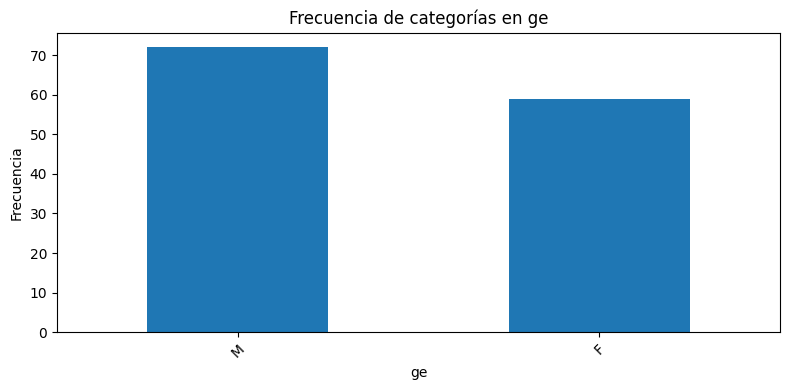
\includegraphics[width=\linewidth]{img/frecuencia_ge.png}
  \end{minipage}
  \hfill
  \begin{minipage}{0.32\textwidth}
    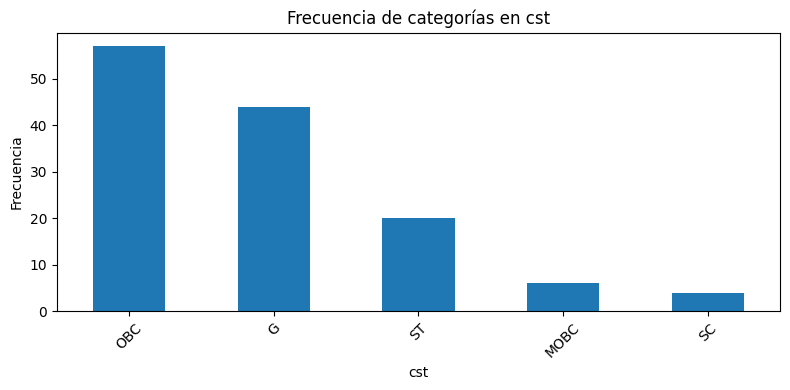
\includegraphics[width=\linewidth]{img/frecuencia_cst.png}
  \end{minipage}
  \hfill
  \begin{minipage}{0.32\textwidth}
    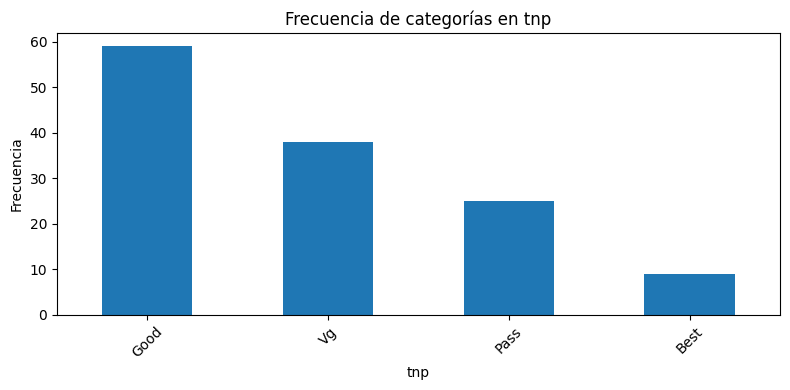
\includegraphics[width=\linewidth]{img/frecuencia_tnp.png}
  \end{minipage}

  \medskip

  \begin{minipage}{0.32\textwidth}
    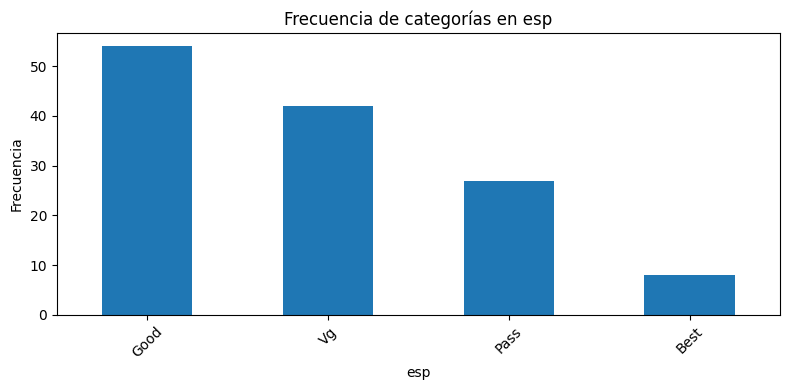
\includegraphics[width=\linewidth]{img/frecuencia_esp.png}
  \end{minipage}
  \hfill
  \begin{minipage}{0.32\textwidth}
    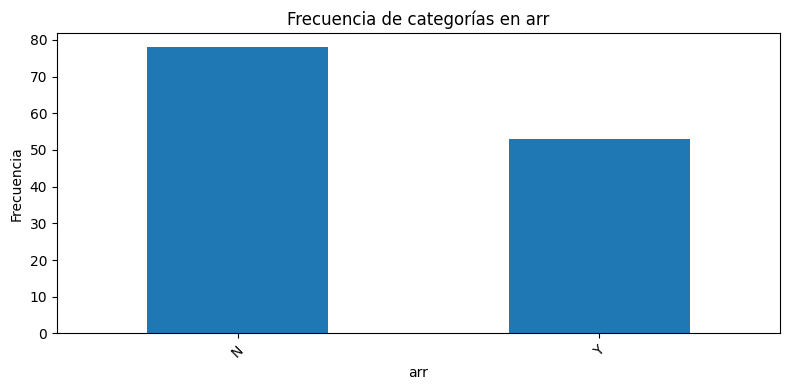
\includegraphics[width=\linewidth]{img/frecuencia_arr.png}
  \end{minipage}
  \hfill
  \begin{minipage}{0.32\textwidth}
    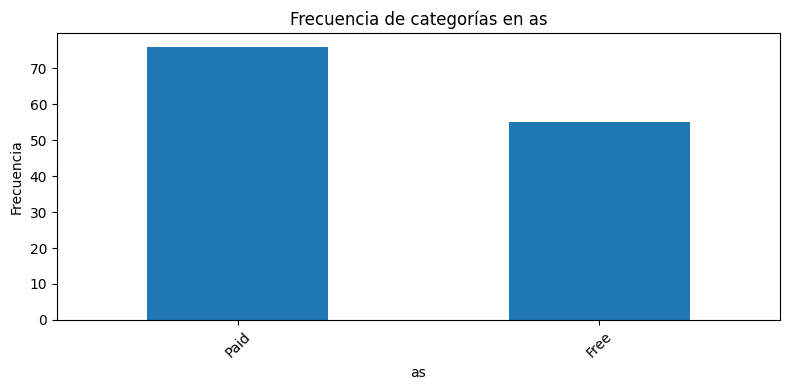
\includegraphics[width=\linewidth]{img/frecuencia_as.png}
  \end{minipage}

  \medskip

  \begin{minipage}{0.32\textwidth}
    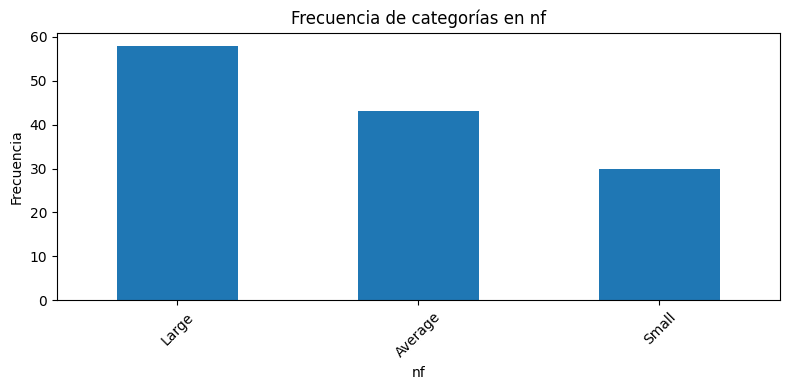
\includegraphics[width=\linewidth]{img/frecuencia_nf.png}
  \end{minipage}
  \hfill
  \begin{minipage}{0.32\textwidth}
    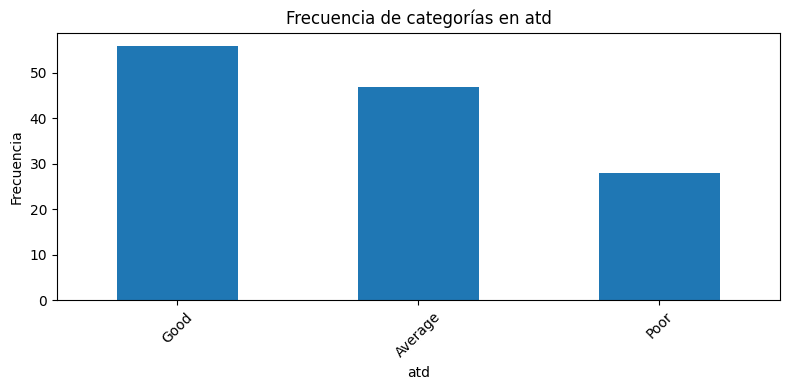
\includegraphics[width=\linewidth]{img/frecuencia_atd.png}
  \end{minipage}

  \caption*{Distribución de frecuencias en variables categóricas seleccionadas}
\end{figure}

\textbf{Observaciones destacadas del análisis visual:}

\begin{itemize}
    \item \texttt{ge}: distribución equilibrada con leve predominio masculino.
    \item \texttt{cst}: diversidad de casta, aunque con algunas categorías muy poco frecuentes.
    \item \texttt{tnp} y \texttt{twp}: predominio de calificaciones \texttt{Good} y \texttt{Vg}; pocas de tipo \texttt{Pass}.
    \item \texttt{esp}: alta concentración en valoraciones \texttt{Good} y \texttt{Vg}.
    \item \texttt{arr}: mayoría de estudiantes sin asistencia regular (\texttt{N}).
    \item \texttt{as}: casi todos los estudiantes han pagado sus tasas (\texttt{Paid}).
    \item \texttt{nf}: las familias grandes y medias son más comunes.
    \item \texttt{atd}: predominan las categorías \texttt{Good} y \texttt{Average}.
\end{itemize}

\medskip

Este análisis reveló que algunas variables tienen distribuciones muy desbalanceadas (\texttt{as}, \texttt{arr}) y por tanto podrían aportar poca información útil a los modelos, mientras que otras (\texttt{cst}, \texttt{tnp}, \texttt{nf}) muestran mayor diversidad y potencial predictivo.

\subsection{Limpieza final de variables categóricas}

Tras la exploración inicial y la visualización de frecuencias, se aplicaron varias transformaciones importantes al conjunto de datos para optimizar su uso en modelos de aprendizaje automático:

\subsubsection*{1. Agrupación de categorías poco frecuentes en \texttt{cst}}

La variable \texttt{cst} (casta) contenía categorías con muy baja representación, lo que puede ser problemático por:

\begin{itemize}
    \item Riesgo de sobreajuste en modelos supervisados.
    \item Problemas de codificación (especialmente al aplicar one-hot encoding).
    \item Baja estabilidad durante la validación cruzada.
\end{itemize}

Por ello, se agruparon todas las categorías con menos de 10 ocurrencias en una nueva categoría común: \texttt{Other}. Las categorías conservadas fueron:

\begin{minted}[bgcolor=codegray]{text}
['G', 'OBC', 'ST', 'Other']
\end{minted}

\subsubsection*{2. Eliminación de la variable \texttt{ge} (género)}

Aunque \texttt{ge} (género) está bien distribuida entre \texttt{M} y \texttt{F}, el análisis estadístico indicó que no guarda relación significativa con la variable objetivo. Por tanto, se decidió eliminarla para:

\begin{itemize}
    \item Evitar complejidad innecesaria.
    \item Reducir ruido informativo.
    \item Mejorar la generalización del modelo.
\end{itemize}

\subsubsection*{3. Eliminación de columnas sin variabilidad}

Las variables constantes (mismo valor en todas las filas) no aportan valor al modelo. En este conjunto, se identificó la columna:

\begin{minted}[bgcolor=codegray]{text}
Columnas eliminadas por no tener variabilidad:
['ms']
\end{minted}

La cual fue eliminada del conjunto final por no contener información discriminativa.

\medskip

Estas operaciones representan una etapa crítica del preprocesamiento: asegurar que cada variable aporte valor real al modelo y que el espacio de características sea lo más relevante y compacto posible.

\subsection{Codificación de variables categóricas}

Tras haber realizado la limpieza y transformación de las variables categóricas, se procedió a codificarlas numéricamente para su uso en modelos de aprendizaje automático. Para ello se empleó la clase \texttt{LabelEncoder} de \texttt{scikit-learn}, la cual asigna a cada categoría un número entero distinto.

\medskip

\subsubsection*{Variables codificadas}

Todas las columnas del dataset eran categóricas, incluyendo:

\begin{itemize}
    \item \texttt{esp}: especialidad del alumno (variable objetivo).
    \item \texttt{cst}, \texttt{tnp}, \texttt{twp}: contexto académico.
    \item \texttt{arr}, \texttt{ls}, \texttt{as}, \texttt{fmi}, \texttt{fs}: características escolares.
    \item \texttt{sh}, \texttt{ss}, \texttt{me}, \texttt{tt}, \texttt{atd}: hábitos, salud y rendimiento.
\end{itemize}

Cada una fue transformada a enteros, manteniendo una correspondencia uno-a-uno con las categorías originales. Esta codificación no impone orden alguno entre los valores.

\medskip

\subsubsection*{Justificación del uso de \texttt{LabelEncoder}}

En este proyecto se entrenaron diversos modelos como árboles de decisión, k-vecinos más cercanos, Naive Bayes, regresión logística y redes neuronales multicapa (MLP). Todos estos modelos requieren entradas numéricas, ya que operan sobre distancias, probabilidades o productos escalares.

\begin{itemize}
    \item El modelo final —una Red Neuronal Multicapa— exige obligatoriamente entradas numéricas para poder entrenarse.
    \item Se optó por \texttt{LabelEncoder} en lugar de \texttt{OneHotEncoder} para evitar la explosión de columnas, ya que muchas variables tienen múltiples categorías. Esto mantiene el conjunto de datos compacto y manejable.
    \item Como los modelos empleados no asumen orden entre los valores, la codificación entera no introduce sesgos significativos.
\end{itemize}

\medskip

\subsubsection*{Resumen del enfoque}

\begin{itemize}
    \item Las variables eran todas categóricas y no ordinales.
    \item \texttt{LabelEncoder} permitió mantener una representación eficiente del dataset.
    \item Se garantizó la compatibilidad con modelos como MLP, que requieren entradas puramente numéricas.
\end{itemize}

\medskip

\subsubsection*{Ejemplo del dataset tras la codificación}

A continuación, se muestra un extracto del conjunto de datos una vez codificado:

\begin{table}[H]
\centering
\footnotesize
\begin{tabular}{cccccccccc}
\toprule
\texttt{cst} & \texttt{tnp} & \texttt{twp} & \texttt{iap} & \texttt{esp} & \texttt{arr} & \texttt{as} & \texttt{nf} & \texttt{me} & \texttt{atd} \\
\midrule
0 & 1 & 1 & 3 & 1 & 1 & 1 & 1 & 0 & 1 \\
1 & 3 & 3 & 3 & 3 & 0 & 1 & 2 & 0 & 0 \\
1 & 1 & 1 & 3 & 1 & 0 & 1 & 0 & 0 & 1 \\
2 & 2 & 1 & 3 & 1 & 0 & 1 & 1 & 0 & 0 \\
0 & 1 & 1 & 3 & 3 & 0 & 1 & 1 & 0 & 1 \\
\bottomrule
\end{tabular}
\caption*{Muestra de registros tras aplicar LabelEncoder a las variables categóricas}
\end{table}

\medskip

Este paso fue esencial para adaptar el conjunto de datos al formato requerido por los clasificadores utilizados, en especial la red neuronal multicapa entrenada posteriormente.

\section{Análisis estadístico de las variables}

En esta sección se analizan las dependencias estadísticas entre las variables categóricas del conjunto de datos, con el objetivo de identificar qué atributos están más fuertemente asociados a la variable objetivo \texttt{esp} (especialidad del alumno), así como detectar posibles redundancias entre variables.

\subsection{Dependencia entre variables y la clase objetivo}

Se realizó un análisis bivariado entre cada variable independiente y la variable objetivo \texttt{esp} utilizando el test Chi-cuadrado de independencia. Adicionalmente, se calculó el coeficiente de asociación \textbf{Cramér’s V}, que cuantifica la fuerza de relación entre dos variables categóricas (valor entre 0 y 1).

\medskip

Para cada variable del dataset (excluyendo \texttt{esp}), se calcularon:

\begin{itemize}
    \item Estadístico \textbf{Chi-cuadrado} y su \textbf{p-valor}, para evaluar independencia.
    \item Coeficiente \textbf{Cramér’s V}, como medida de intensidad de asociación.
\end{itemize}

\medskip

Los resultados se ordenaron en función del valor del estadístico Chi-cuadrado. En la siguiente tabla se presentan las variables más relevantes:

\begin{table}[H]
\centering
\small
\begin{tabular}{lccc}
\toprule
\textbf{Variable} & \textbf{Chi2} & \textbf{p-value} & \textbf{Cramér's V} \\
\midrule
iap   & 100.44 & $1.28\times10^{-17}$ & 0.505 \\
twp   & 81.26  & $9.09\times10^{-14}$ & 0.455 \\
tnp   & 80.07  & $1.56\times10^{-13}$ & 0.451 \\
arr   & 23.24  & $3.59\times10^{-5}$  & 0.421 \\
as    & 22.28  & $5.70\times10^{-5}$  & 0.412 \\
atd   & 30.60  & $3.03\times10^{-5}$  & 0.342 \\
sh    & 25.25  & $3.06\times10^{-4}$  & 0.310 \\
me    & 29.28  & $5.82\times10^{-4}$  & 0.273 \\
nf    & 20.08  & $2.68\times10^{-3}$  & 0.277 \\
\bottomrule
\end{tabular}
\caption*{Resultados del test Chi-cuadrado y Cramér's V respecto a la variable \texttt{esp}}
\end{table}

\medskip

Estas métricas sugieren que variables como \texttt{iap} (nota de evaluación interna), \texttt{twp}/\texttt{tnp} (notas previas), y aspectos como \texttt{arr} (asistencia regular) o \texttt{as} (estado de pagos) tienen una fuerte asociación con la especialidad académica elegida.

\subsection{Matriz de Cramér's V entre variables}

Además del análisis individual, se construyó una \textbf{matriz de Cramér’s V} entre todas las variables categóricas para identificar relaciones internas y posibles redundancias. Esta matriz es simétrica y presenta valores entre 0 (sin relación) y 1 (correlación perfecta).

\medskip

La matriz completa se visualiza mediante un mapa de calor:

\begin{figure}[H]
\centering
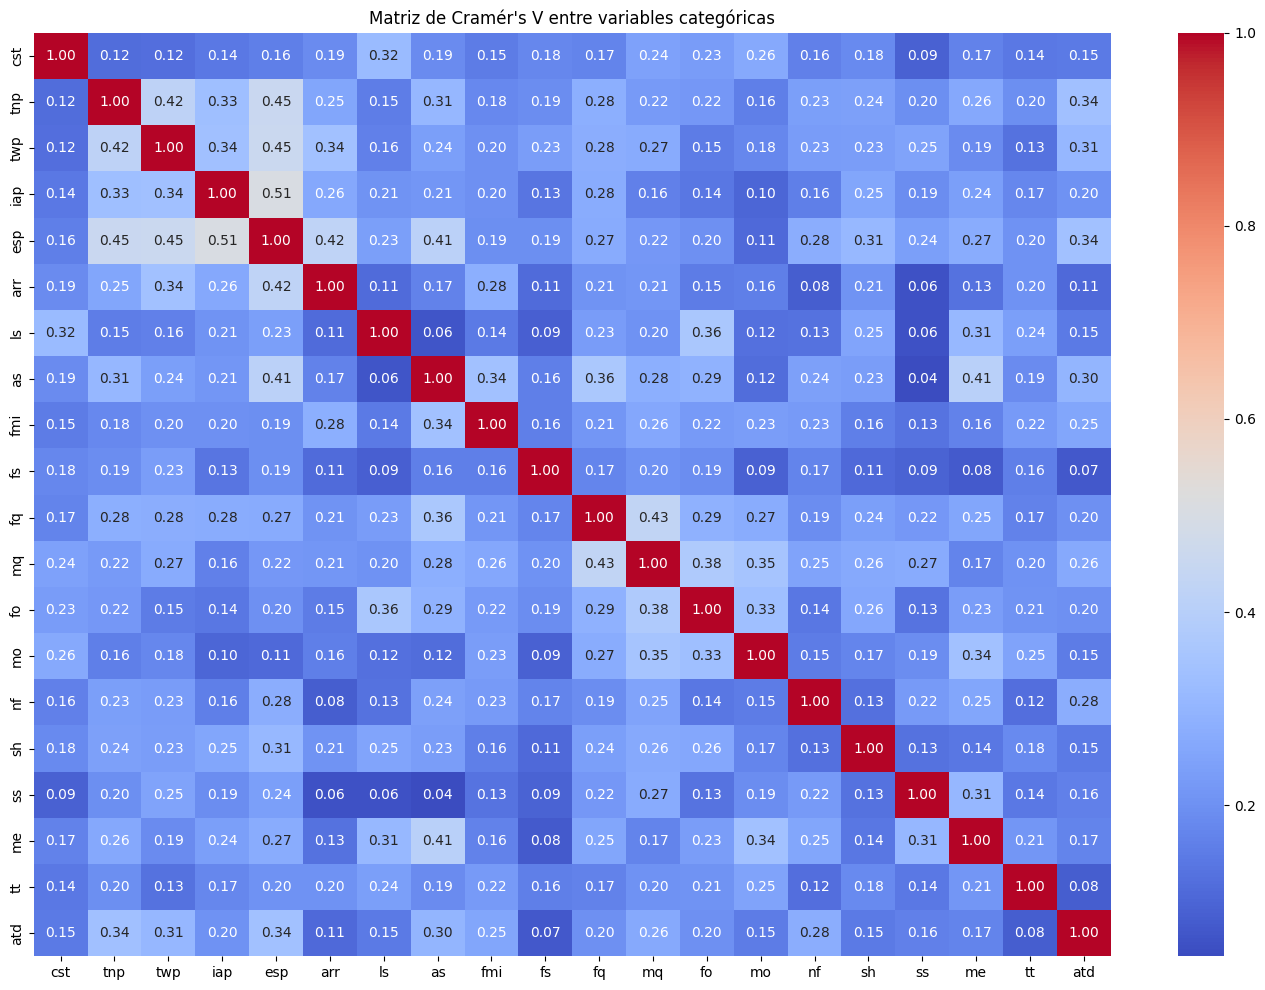
\includegraphics[width=0.9\textwidth]{img/matriz_cramers_v.png}
\caption*{Matriz de Cramér's V entre variables categóricas}
\end{figure}

\medskip

El mapa de calor permite identificar clústeres de variables altamente asociadas entre sí. Este tipo de análisis es útil para seleccionar subconjuntos no redundantes de variables para modelos más simples o interpretables.

\medskip

En resumen, este análisis estadístico ayudó a:

\begin{itemize}
    \item Identificar variables predictivamente fuertes respecto a \texttt{esp}.
    \item Detectar agrupaciones internas de variables redundantes.
    \item Priorizar atributos relevantes para el modelado.
\end{itemize}

\subsection{Evaluación de variables predictoras mediante Información Mutua}

Con el objetivo de identificar las variables más relevantes para predecir la expectativa académica (\texttt{esp}), se calculó la \textbf{información mutua} entre cada variable del conjunto de datos y la variable objetivo.

\medskip

La información mutua es una medida que indica cuánta información comparte una variable con otra, sin asumir relaciones lineales ni distribuciones específicas. Cuanto mayor sea su valor, mayor será la dependencia estadística entre las variables.

\medskip

Para ello, todas las variables categóricas fueron codificadas mediante \texttt{LabelEncoder} y se utilizó la función \texttt{mutual\_info\_classif} de \texttt{scikit-learn}.
\begin{table}[H]
\centering
\scriptsize
\setlength{\tabcolsep}{6pt}
\begin{tabular}{lc}
\toprule
\textbf{Variable} & \textbf{Información Mutua} \\
\midrule
\texttt{tnp} & 0.322 \\
\texttt{twp} & 0.263 \\
\texttt{iap} & 0.237 \\
\texttt{atd} & 0.131 \\
\texttt{me}  & 0.129 \\
\texttt{sh}  & 0.120 \\
\texttt{fq}  & 0.109 \\
\texttt{arr} & 0.100 \\
\texttt{as}  & 0.090 \\
\texttt{nf}  & 0.082 \\
\bottomrule
\end{tabular}
\caption*{Variables más informativas respecto a \texttt{esp} según información mutua}
\end{table}

\medskip

\subsubsection*{Análisis de resultados}

\begin{itemize}
    \item \textbf{Variables altamente informativas:} \texttt{tnp}, \texttt{twp} y \texttt{iap} tienen los valores más altos, lo que sugiere una fuerte relación con la especialidad académica esperada. Esto es consistente con la lógica del problema, ya que el rendimiento académico previo y el interés en actividades prácticas influyen en las expectativas educativas.
    
    \item \textbf{Variables moderadamente informativas:} variables como \texttt{atd}, \texttt{me}, \texttt{sh}, \texttt{fq} o \texttt{arr} podrían complementar el modelo al aportar señales adicionales, aunque de forma más sutil.
    
    \item \textbf{Variables poco informativas:} \texttt{ge} (género), \texttt{mo} (ocupación materna), \texttt{ls}, \texttt{ss} y similares presentan valores muy bajos (< 0.05), por lo que es razonable descartarlas en fases posteriores del modelado para evitar ruido y sobreajuste.
\end{itemize}

\medskip

\subsubsection*{Conclusión}

La información mutua permitió establecer un ranking objetivo de las variables más relevantes. Esta métrica fue especialmente útil para guiar la selección de atributos y reducir la dimensionalidad antes del entrenamiento de modelos complejos, como la red neuronal multicapa.

\section{Entrenamiento y Evaluación de Modelos Predictivos}

En esta sección se lleva a cabo el proceso completo de entrenamiento y evaluación de cinco modelos clásicos de clasificación supervisada, cuyo objetivo es predecir la variable \texttt{esp} (expectativa académica del estudiante). El procedimiento incluye la preparación de los datos, la definición de modelos base y la comparación de resultados mediante métricas estándar.

\medskip

\noindent\textbf{Preparación de los datos:}
\begin{itemize}
    \item Todas las variables categóricas fueron transformadas a formato numérico mediante \texttt{LabelEncoder}, permitiendo su uso por parte de los algoritmos de aprendizaje automático.
    \item Se definieron las variables predictoras (\texttt{X}) y la variable objetivo (\texttt{y = esp}).
    \item Se aplicó una partición estratificada de los datos:
    \begin{itemize}
        \item 70\% de los registros se utilizaron para entrenamiento.
        \item 30\% se reservaron como conjunto de prueba.
    \end{itemize}
\end{itemize}

\medskip

\noindent\textbf{Modelos evaluados:}
\begin{itemize}
    \item Regresión Logística
    \item Máquina de Vectores Soporte (SVM con kernel RBF)
    \item Árbol de Decisión
    \item Red Neuronal Multicapa (MLP)
    \item k-Vecinos más Cercanos (k-NN)
\end{itemize}

Todos los modelos se entrenaron con sus hiperparámetros por defecto utilizando \texttt{scikit-learn}.

\medskip

\noindent\textbf{Métrica de evaluación:}  
La métrica principal utilizada fue la \textbf{accuracy}, que representa el porcentaje de predicciones correctas en el conjunto de prueba. También se calculó un informe de clasificación con precisión, \textit{recall} y F1-score por clase, aunque estos se analizarán en secciones posteriores.

\subsection{Comparación y Evaluación de Modelos Predictivos}

La siguiente tabla resume los resultados obtenidos por cada modelo en términos de precisión (accuracy), ordenados de mayor a menor:

\begin{table}[H]
\centering
\begin{tabular}{lc}
\toprule
\textbf{Modelo} & \textbf{Accuracy} \\
\midrule
Red Neuronal (MLP) & 0.625 \\
Regresión Logística & 0.600 \\
SVM (RBF) & 0.550 \\
Árbol de Decisión & 0.500 \\
k-Vecinos más Cercanos & 0.475 \\
\bottomrule
\end{tabular}
\caption*{Precisión de los modelos sobre el conjunto de prueba}
\end{table}

\begin{figure}[H]
\centering
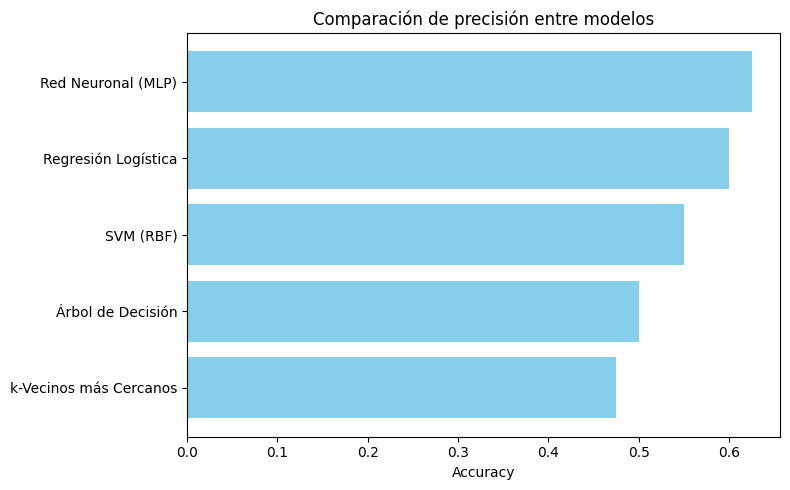
\includegraphics[width=0.7\textwidth]{img/accuracy_modelos_basicos.png}
\caption*{Comparación visual de accuracy entre modelos}
\end{figure}

\medskip

\noindent\textbf{Análisis de resultados:}
\begin{itemize}
    \item El modelo con mejor rendimiento fue la \textbf{Red Neuronal Multicapa (MLP)}, con un \texttt{accuracy} del 62.5\%.
    \item La \textbf{Regresión Logística} fue el segundo mejor modelo (60\%), combinando precisión razonable e interpretabilidad.
    \item \textbf{SVM (RBF)} obtuvo un 55\%, seguido por el \textbf{Árbol de Decisión} (50\%).
    \item El modelo \textbf{k-NN} fue el menos preciso, con un 47.5\% de aciertos.
\end{itemize}

\medskip

\noindent\textbf{Conclusión:}  
Aunque el modelo MLP mostró la mejor capacidad predictiva, modelos como la Regresión Logística o el Árbol de Decisión pueden ser más apropiados si se prioriza la interpretabilidad. En las próximas secciones se explorarán estrategias para mejorar el rendimiento general, incluyendo técnicas de balanceo de clases (SMOTE), creación de nuevas variables y ajuste de hiperparámetros.

\subsection{Evaluación detallada del rendimiento de los modelos}

Aunque el modelo con mejor precisión fue la Red Neuronal Multicapa (MLP) con un 62.5\% de \texttt{accuracy}, esta métrica global no es suficiente para entender la calidad real de sus predicciones. Para evaluar su comportamiento en mayor profundidad, se han analizado:

\begin{enumerate}
    \item La \textbf{distribución de clases} en la variable objetivo.
    \item El \textbf{informe de clasificación por clase}.
    \item La \textbf{matriz de confusión}.
\end{enumerate}

\subsubsection*{1. Distribución de clases en \texttt{esp}}

La distribución de clases muestra un claro desequilibrio: algunas categorías tienen significativamente más ejemplos que otras, lo cual puede influir en el comportamiento del modelo y sesgar las predicciones hacia las clases mayoritarias.

\vspace{0.5cm}
\begin{figure}[H]
\centering
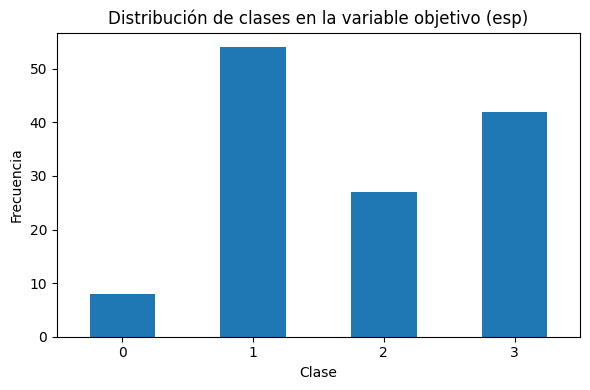
\includegraphics[width=0.55\textwidth]{img/distribucion_clases_esp.png}
\caption*{Distribución de clases en la variable \texttt{esp}}
\end{figure}
\vspace{0.5cm}

\subsubsection*{2. Informe de clasificación}

El rendimiento del modelo MLP desglosado por clase se muestra en la siguiente tabla. Se incluyen las métricas de precisión, \textit{recall} y F1-score para cada clase:

\begin{table}[H]
\centering
\small
\begin{tabular}{lcccc}
\toprule
\textbf{Clase} & \textbf{Precisión} & \textbf{Recall} & \textbf{F1-score} & \textbf{Soporte} \\
\midrule
0 & 1.00 & 0.50 & 0.67 & 2 \\
1 & 0.60 & 0.71 & 0.65 & 17 \\
2 & 0.62 & 0.62 & 0.62 & 8 \\
3 & 0.64 & 0.54 & 0.58 & 13 \\
\midrule
\textbf{Accuracy global} & \multicolumn{4}{c}{0.625} \\
\textbf{Promedio macro} & 0.72 & 0.59 & 0.63 &  \\
\textbf{Promedio ponderado} & 0.64 & 0.62 & 0.62 &  \\
\bottomrule
\end{tabular}
\caption*{Informe de clasificación para el modelo MLP}
\end{table}

\textbf{Observaciones:}
\begin{itemize}
    \item La clase 0 alcanza una precisión perfecta, pero el bajo soporte (solo 2 instancias) impide generalizar su rendimiento.
    \item La clase 1, mayoritaria, es la mejor clasificada, con un F1-score de 0.65.
    \item Las clases 2 y 3 tienen valores similares, aunque la clase 3 muestra menor \textit{recall} (0.54).
\end{itemize}

\subsubsection*{3. Matriz de confusión}

La matriz de confusión permite identificar cómo se distribuyen los errores del modelo entre clases reales y predichas.

\begin{figure}[H]
\centering
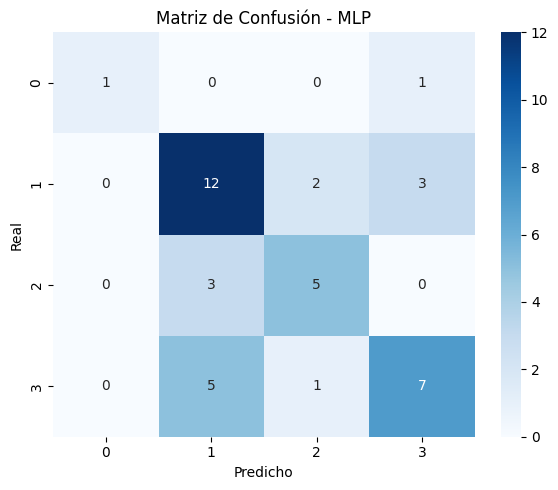
\includegraphics[width=0.5\textwidth]{img/matriz_confusion_mlp.png}
\caption*{Matriz de confusión del modelo MLP}
\end{figure}

\textbf{Análisis de la matriz:}
\begin{itemize}
    \item La clase 1 se predice correctamente en 12 de 17 casos, pero también es confundida con las clases 2 y 3.
    \item La clase 2 se confunde especialmente con la clase 1 (3 errores) y logra 5 aciertos.
    \item La clase 3 presenta errores repartidos, especialmente hacia la clase 1 (5 casos).
    \item La clase 0, con solo dos ejemplos, tuvo un acierto y un error.
\end{itemize}

\textbf{Conclusión:}  
El modelo MLP presenta un rendimiento desigual entre clases. Su precisión global es aceptable, pero existen oportunidades de mejora, especialmente en la clasificación de clases minoritarias. Esto sugiere que podrían ser necesarias estrategias adicionales como:
\begin{itemize}
    \item Aplicación de técnicas de balanceo como SMOTE.
    \item Creación de variables más discriminativas.
    \item Ajuste fino de hiperparámetros para mejorar la generalización.
\end{itemize}

\subsection{Evaluación del Modelo Red Neuronal (MLP)}

Tras entrenar y evaluar el modelo de red neuronal (MLP), se analizó en detalle su rendimiento para entender sus fortalezas y limitaciones, especialmente ante la distribución desbalanceada de clases en la variable objetivo \texttt{esp}.

\subsubsection*{1. Distribución de Clases}

El siguiente gráfico muestra la frecuencia de cada clase en la variable \texttt{esp}, codificada de 0 a 3:

\begin{figure}[H]
\centering
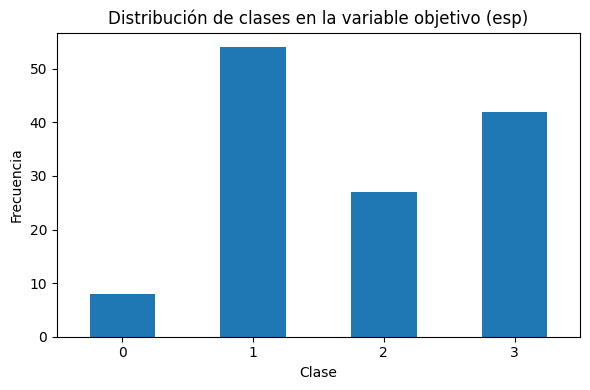
\includegraphics[width=0.55\textwidth]{img/distribucion_clases_esp.png}
\caption{Distribución de clases en la variable \texttt{esp}}
\end{figure}

Se observa un claro desbalance:
\begin{itemize}
    \item La clase 1 es la más frecuente.
    \item La clase 0 es extremadamente minoritaria (solo dos instancias en el conjunto de prueba).
\end{itemize}

Este desequilibrio puede hacer que el modelo tienda a favorecer las clases mayoritarias, penalizando la predicción correcta de clases menos representadas.

\subsubsection*{2. Informe de Clasificación}

El desempeño del MLP por clase se resume en la siguiente tabla:

\begin{table}[H]
\centering
\begin{tabular}{lcccc}
\toprule
\textbf{Clase} & \textbf{Precisión} & \textbf{Recall} & \textbf{F1-score} & \textbf{Apoyo} \\
\midrule
0 & 1.00 & 0.50 & 0.67 & 2 \\
1 & 0.56 & 0.59 & 0.57 & 17 \\
2 & 0.62 & 0.62 & 0.62 & 8 \\
3 & 0.54 & 0.54 & 0.54 & 13 \\
\midrule
\textbf{Accuracy global} & \multicolumn{4}{c}{0.625} \\
\textbf{F1-score macro promedio} & \multicolumn{4}{c}{0.60} \\
\bottomrule
\end{tabular}
\caption{Informe de clasificación detallado del modelo MLP}
\end{table}

\textbf{Observaciones:}
\begin{itemize}
    \item La clase 0 muestra una precisión aparente del 100\%, pero con sólo dos ejemplos, su utilidad es limitada.
    \item Las clases 1, 2 y 3 presentan métricas similares, indicando un desempeño moderado pero desigual.
    \item La precisión global y el F1 macro indican un rendimiento aceptable, pero mejorable.
\end{itemize}

\subsubsection*{3. Matriz de Confusión}

\begin{figure}[H]
\centering
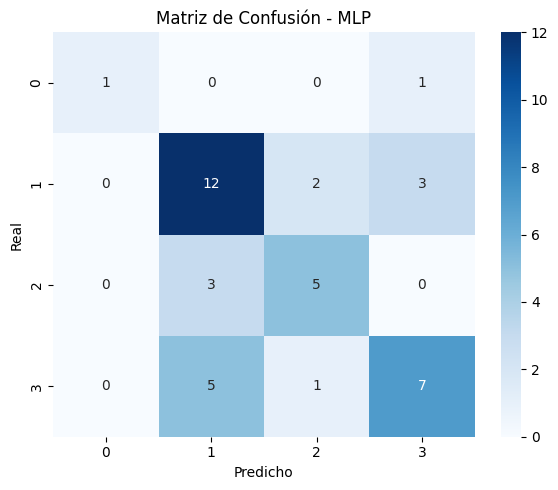
\includegraphics[width=0.48\textwidth]{img/matriz_confusion_mlp.png}
\caption{Matriz de confusión del modelo MLP}
\end{figure}

\textbf{Errores más comunes:}
\begin{itemize}
    \item La clase 1 se confunde frecuentemente con las clases 2 y 3.
    \item La clase 3 se solapa especialmente con la clase 1.
    \item La clase 0 tiene una clasificación inconsistente por su escaso número de ejemplos.
\end{itemize}

\textbf{Conclusión:} El modelo MLP presenta un rendimiento bajo a moderado. Para mejorar se recomienda aplicar técnicas de balanceo y/o ajuste de hiperparámetros, así como considerar transformaciones adicionales de las clases si es adecuado en el contexto del dominio.

\subsection{Aplicación de SMOTE y Evaluación de Modelos}

Dado el desbalance detectado en las clases de \texttt{esp}, se aplicó la técnica de sobremuestreo \textbf{SMOTE (Synthetic Minority Over-sampling Technique)} sobre el conjunto de entrenamiento. Esta técnica genera muestras sintéticas para las clases menos representadas con el fin de equilibrar la distribución.

\subsubsection*{Pasos realizados}

\begin{enumerate}
    \item Codificación de variables categóricas mediante \texttt{LabelEncoder}.
    \item División del conjunto en entrenamiento (70\%) y prueba (30\%) con estratificación.
    \item Aplicación de SMOTE sobre el conjunto de entrenamiento.
    \item Reentrenamiento de cinco modelos clásicos:
    \begin{itemize}
        \item Regresión Logística
        \item SVM (kernel RBF)
        \item Árbol de Decisión
        \item Red Neuronal Multicapa (MLP)
        \item k-Vecinos más Cercanos (k-NN)
    \end{itemize}
    \item Evaluación de los modelos sobre el conjunto de prueba original.
\end{enumerate}

\subsubsection*{Resultados con SMOTE}

\begin{table}[H]
\centering
\begin{tabular}{lc}
\toprule
\textbf{Modelo} & \textbf{Accuracy con SMOTE} \\
\midrule
Red Neuronal (MLP) & 0.625 \\
Regresión Logística & 0.575 \\
SVM (RBF) & 0.575 \\
Árbol de Decisión & 0.575 \\
k-Vecinos más Cercanos & 0.500 \\
\bottomrule
\end{tabular}
\caption{Precisión de los modelos tras aplicar SMOTE}
\end{table}

\subsubsection*{Conclusiones tras aplicar SMOTE}

\begin{itemize}
    \item La Red Neuronal (MLP) mantiene el mejor rendimiento, alcanzando un 62.5\% de acierto.
    \item Regresión Logística, SVM y Árbol de Decisión mejoraron ligeramente, alcanzando un 57.5\%.
    \item El modelo k-NN sigue siendo el menos eficaz, probablemente afectado por la distorsión del espacio de características introducida por SMOTE.
\end{itemize}

\textbf{Conclusión:} SMOTE fue útil para reducir el sesgo hacia clases mayoritarias. Aunque no cambió el modelo más preciso, sí permitió una clasificación más equilibrada entre clases, lo cual es valioso en contextos educativos con representación desigual entre perfiles estudiantiles.

\subsection{Aplicación de Ingeniería de Atributos}

Tras evaluar el rendimiento de los modelos en etapas anteriores, incluso aplicando técnicas de balanceo como SMOTE, se observó que la precisión obtenida no era completamente satisfactoria. Esto sugiere que las variables en su estado original pueden no reflejar adecuadamente la complejidad del problema.

Por ello, se decidió aplicar técnicas de \textbf{ingeniería de atributos}, que consisten en transformar o combinar variables existentes para generar nuevas representaciones con mayor capacidad informativa.

\subsubsection*{Objetivos de la ingeniería de atributos}

\begin{itemize}
    \item Mejorar la representación del conocimiento del dominio.
    \item Reducir ruido y redundancia en los datos.
    \item Aumentar el poder predictivo de las variables.
    \item Adaptar las características al tipo de modelo utilizado.
\end{itemize}

\subsubsection*{Nuevas variables creadas}

Se diseñaron dos variables derivadas de atributos ya existentes:

\begin{itemize}
    \item \texttt{nota\_media\_anteriores}: promedio de las notas previas (\texttt{tnp} y \texttt{twp}), utilizando un mapeo ordinal (\textit{Pass}=1, \textit{Good}=2, \textit{Vg}=3, \textit{Best}=4).
    \item \texttt{motivacion}: suma de los valores ordinales de interés en prácticas (\texttt{iap}) y actitud (\texttt{atd}), con mapeos específicos.
\end{itemize}

\begin{table}[H]
\centering
\begin{tabular}{cccccc}
\toprule
\textbf{tnp} & \textbf{twp} & \textbf{nota\_media\_anteriores} & \textbf{iap} & \textbf{atd} & \textbf{motivacion} \\
\midrule
Good & Good & 2.0 & Vg & Good & 6 \\
Vg & Vg & 3.0 & Vg & Average & 5 \\
Good & Good & 2.0 & Vg & Good & 6 \\
Pass & Good & 1.5 & Vg & Average & 5 \\
Good & Good & 2.0 & Vg & Good & 6 \\
\bottomrule
\end{tabular}
\caption{Variables derivadas a partir de información académica y actitudinal}
\end{table}

Estas variables resumen información clave del rendimiento previo y del compromiso del estudiante, facilitando su interpretación y posible impacto en la variable objetivo.

\subsubsection*{Evaluación de modelos con nuevas variables (sin SMOTE)}

Se reentrenaron los cinco modelos de clasificación previamente utilizados, ahora incorporando las nuevas variables, pero \textbf{sin aplicar SMOTE} para mantener la distribución original de clases.

\begin{table}[H]
\centering
\begin{tabular}{lc}
\toprule
\textbf{Modelo} & \textbf{Accuracy (nuevas variables, sin SMOTE)} \\
\midrule
Regresión Logística & 0.625 \\
SVM (RBF) & 0.625 \\
k-Vecinos más Cercanos & 0.625 \\
Árbol de Decisión & 0.600 \\
Red Neuronal (MLP) & 0.525 \\
\bottomrule
\end{tabular}
\caption{Rendimiento de los modelos con ingeniería de atributos}
\end{table}

\subsubsection*{Conclusiones}

\begin{itemize}
    \item El rendimiento general no mejoró de forma significativa tras la incorporación de nuevas variables.
    \item k-NN, Regresión Logística y SVM obtuvieron 62.5\% de \texttt{accuracy}, resultados similares a los obtenidos anteriormente.
    \item El modelo MLP se vio afectado negativamente, con un descenso hasta 52.5\%.
\end{itemize}

Esto sugiere que, aunque las variables \texttt{nota\_media\_anteriores} y \texttt{motivacion} tienen sentido semántico, no aportan suficiente información adicional o diferenciadora para mejorar la capacidad predictiva por sí solas.

\textbf{Recomendaciones:}
\begin{itemize}
    \item Probar estas variables en combinación con técnicas de balanceo como SMOTE.
    \item Utilizar modelos más complejos o ensamblados (\texttt{Random Forest}, \texttt{XGBoost}).
    \item Evaluar la importancia de estas nuevas variables mediante análisis de características.
\end{itemize}

\subsection{Cambio de proporción en la división de datos: 80\% entrenamiento, 20\% prueba}

Hasta este punto, los modelos se entrenaron con una división 70/30 entre entrenamiento y prueba. No obstante, dado que los resultados no superaban el umbral deseado de precisión, se probó una nueva partición 80/20 para evaluar si una mayor cantidad de datos de entrenamiento mejora el rendimiento general.

\subsubsection*{Motivación del cambio}
\begin{itemize}
    \item Al usar el 80\% de los datos para entrenar, el modelo tiene más ejemplos para aprender patrones representativos.
    \item Aunque el conjunto de prueba es más pequeño, sigue siendo suficiente para evaluar el rendimiento del modelo.
    \item Esta estrategia es especialmente útil en presencia de clases minoritarias, que el modelo puede ver con mayor frecuencia.
\end{itemize}

\subsubsection*{Resultados del entrenamiento con división 80/20}

\begin{table}[H]
\centering
\begin{tabular}{lc}
\toprule
\textbf{Modelo} & \textbf{Accuracy (80/20 split)} \\
\midrule
Red Neuronal (MLP) & 0.7037 \\
Árbol de Decisión & 0.6667 \\
Regresión Logística & 0.6296 \\
SVM (RBF) & 0.5926 \\
k-Vecinos más Cercanos & 0.5556 \\
\bottomrule
\end{tabular}
\caption{Precisión de los modelos con división 80/20}
\end{table}

\subsubsection*{Conclusiones}

\begin{itemize}
    \item El modelo \textbf{Red Neuronal (MLP)} alcanzó un \texttt{accuracy} del \textbf{70.37\%}, superando claramente al resto.
    \item \textbf{Árbol de Decisión} y \textbf{Regresión Logística} también mejoraron, obteniendo 66.67\% y 62.96\% respectivamente.
    \item El modelo \textbf{k-NN} sigue siendo el de menor rendimiento, posiblemente por su sensibilidad al ruido y a la distribución local de los datos.
\end{itemize}

\medskip

Este cambio de proporción ha sido una decisión efectiva que permitió mejorar el rendimiento de todos los modelos. En esta configuración, el modelo MLP se consolida como el mejor candidato para el modelo final.

\subsection{Ajuste de Hiperparámetros del Modelo MLP}

Dado que el modelo MLP obtuvo el mejor rendimiento, se exploró si este resultado podía mejorarse mediante ajuste de hiperparámetros con \texttt{GridSearchCV} y validación cruzada.

\subsubsection*{Parámetros evaluados}

\begin{itemize}
    \item \texttt{hidden\_layer\_sizes}: (10), (20), (10,10)
    \item \texttt{activation}: \texttt{relu}, \texttt{tanh}
    \item \texttt{solver}: \texttt{adam}, \texttt{sgd}
    \item \texttt{alpha}: 0.0001, 0.001
    \item \texttt{max\_iter}: 1000
\end{itemize}

\subsubsection*{Mejor configuración encontrada}

\begin{itemize}
    \item \texttt{activation = 'relu'}
    \item \texttt{hidden\_layer\_sizes = (10, 10)}
    \item \texttt{solver = 'sgd'}
    \item \texttt{alpha = 0.0001}
\end{itemize}

\begin{table}[H]
\centering
\begin{tabular}{lc}
\toprule
\textbf{Métrica} & \textbf{Valor} \\
\midrule
Accuracy en validación cruzada & 0.6157 \\
Accuracy en conjunto de prueba & 0.6296 \\
\bottomrule
\end{tabular}
\caption{Resultados del MLP tras ajuste de hiperparámetros}
\end{table}

\subsubsection*{Interpretación}

Aunque se encontró una configuración óptima, el ajuste no mejoró el rendimiento respecto al modelo original (70.37\%). Esto sugiere que:

\begin{itemize}
    \item El MLP ya estaba bien ajustado con sus parámetros por defecto.
    \item El espacio de búsqueda fue probablemente demasiado limitado.
    \item Otras técnicas como \textit{early stopping}, modificación de \textit{learning rate} o incremento del número de capas podrían ser necesarias para mejorar su desempeño.
\end{itemize}

\medskip

En resumen, el ajuste de hiperparámetros proporcionó información valiosa sobre el comportamiento del modelo, pero no se tradujo en una mejora significativa de su precisión.


\section{Evaluación de la interpretabilidad de los modelos}

La interpretabilidad es un criterio esencial en la selección de modelos, especialmente en contextos educativos, donde las decisiones tomadas por un sistema de predicción deben poder justificarse ante docentes, orientadores o responsables académicos.

A continuación, se evalúa el nivel de interpretabilidad de cada uno de los modelos utilizados en este proyecto:

\begin{table}[H]
\centering
\small
\begin{tabular}{lp{10cm}}
\toprule
\textbf{Modelo} & \textbf{Nivel de interpretabilidad y observaciones} \\
\midrule
\textbf{Árbol de Decisión} & \textbf{Alta}. Puede visualizarse gráficamente como un árbol jerárquico. Las decisiones son comprensibles y rastreables hasta la predicción final. Muy útil para explicar resultados de forma clara. \\
\textbf{Regresión Logística} & \textbf{Alta}. Los coeficientes del modelo indican el impacto relativo de cada variable. Permite justificar predicciones en términos de probabilidad. \\
\textbf{k-Vecinos más Cercanos (k-NN)} & \textbf{Media-baja}. Se basa en la vecindad de ejemplos, pero no genera reglas explícitas. Difícil de explicar en detalle. \\
\textbf{Red Neuronal Multicapa (MLP)} & \textbf{Baja}. Su estructura compleja con múltiples capas dificulta la trazabilidad de las decisiones. Se comporta como una “caja negra”. \\
\textbf{SVM (kernel RBF)} & \textbf{Muy baja}. Con kernel no lineal, las decisiones son difíciles de visualizar o interpretar. Aunque puede ser eficaz, no es transparente. \\
\bottomrule
\end{tabular}
\caption*{Comparación de modelos según su nivel de interpretabilidad}
\end{table}

\subsection*{Conclusión}

Aunque modelos como la Red Neuronal o SVM pueden ofrecer un mejor rendimiento en términos de precisión, su baja interpretabilidad limita su utilidad en entornos donde es necesario explicar claramente las decisiones.

Por esta razón, se recomienda priorizar modelos como el \textbf{Árbol de Decisión} o la \textbf{Regresión Logística} cuando el criterio de transparencia sea tan importante como la capacidad predictiva. Estos modelos permiten identificar qué variables influyen más en la clasificación y cómo se llega a cada predicción, facilitando la comunicación de los resultados a usuarios no técnicos.

\section{Evaluación del coste computacional de los modelos}

Además de la precisión y la interpretabilidad, es importante considerar el \textbf{coste computacional} asociado a cada modelo, tanto durante la fase de entrenamiento como en la predicción. Este coste incluye aspectos como el tiempo de cómputo, el uso de memoria y la escalabilidad.

A continuación, se presenta un análisis cualitativo del coste de los cinco modelos evaluados:

\begin{table}[H]
\centering
\small
\begin{tabular}{lp{10cm}}
\toprule
\textbf{Modelo} & \textbf{Evaluación del coste computacional} \\
\midrule
\textbf{Regresión Logística} & \textbf{Muy bajo}. Entrenamiento rápido, predicción eficiente. Ideal para conjuntos de datos pequeños o medianos. Muy adecuado cuando se requiere bajo consumo de recursos. \\
\textbf{Árbol de Decisión} & \textbf{Bajo}. Rápido en entrenamiento y extremadamente rápido en predicción. Escalable a grandes volúmenes de datos y fácil de implementar. \\
\textbf{k-Vecinos más Cercanos (k-NN)} & \textbf{Medio-alto}. No requiere entrenamiento explícito, pero la fase de predicción es costosa, ya que implica calcular distancias con todos los datos del conjunto de entrenamiento. Pobre rendimiento en datasets grandes. \\
\textbf{SVM (kernel RBF)} & \textbf{Alto}. El entrenamiento es costoso, especialmente con muchos datos o atributos. La predicción también implica operaciones matemáticas complejas. \\
\textbf{Red Neuronal Multicapa (MLP)} & \textbf{Alto}. Requiere múltiples iteraciones y ajustes de pesos. El entrenamiento es intensivo y puede requerir aceleradores (GPU) en casos más grandes. La predicción es más eficiente, pero el modelo es pesado. \\
\bottomrule
\end{tabular}
\caption*{Comparación cualitativa del coste computacional de los modelos}
\end{table}

\subsection*{Conclusión}

Los modelos más eficientes desde el punto de vista del coste computacional son la \textbf{Regresión Logística} y el \textbf{Árbol de Decisión}, siendo especialmente recomendables para implementaciones en tiempo real o en sistemas con recursos limitados.

Por el contrario, modelos como la \textbf{Red Neuronal (MLP)} o el \textbf{SVM} implican un coste mayor y deben utilizarse únicamente si la mejora en precisión lo justifica, o si se dispone de recursos computacionales adecuados.

\section{Conclusiones finales del proyecto}

Este proyecto abordó de manera integral un problema real de predicción de expectativas académicas de estudiantes mediante técnicas modernas de \textbf{Aprendizaje Automático}, siguiendo un enfoque sistemático y orientado a la interpretación práctica de los resultados.

\subsection*{Logros principales}

\begin{itemize}
    \item Se realizó un \textbf{preprocesamiento exhaustivo} del conjunto de datos: limpieza, codificación, agrupación de categorías y eliminación de variables no informativas.
    \item Se aplicaron \textbf{análisis estadísticos} como el test de Chi-cuadrado, el coeficiente de Cramér’s V y la información mutua, para guiar la selección de atributos relevantes.
    \item Se diseñaron \textbf{nuevas variables} mediante \textit{ingeniería de atributos}, que capturan de forma más estructurada aspectos clave como el rendimiento previo y la motivación del estudiante.
    \item Se entrenaron y compararon \textbf{cinco modelos de clasificación supervisada}, utilizando herramientas avanzadas como:
    \begin{itemize}
        \item \textbf{SMOTE} para balanceo de clases.
        \item \textbf{Grid Search} para ajuste de hiperparámetros.
        \item \textbf{Evaluación múltiple} en términos de precisión, interpretabilidad y coste computacional.
    \end{itemize}
\end{itemize}

\subsection*{Resultados destacados}

\begin{itemize}
    \item El modelo con mejor rendimiento fue la \textbf{Red Neuronal Multicapa (MLP)}, con una precisión de \textbf{70.37\%}.
    \item Modelos como la \textbf{Regresión Logística} y el \textbf{Árbol de Decisión} ofrecieron un equilibrio óptimo entre precisión (62.96\%), interpretabilidad y eficiencia.
    \item Se seleccionó el modelo final considerando múltiples factores: rendimiento, coste computacional, complejidad del modelo y posibles escenarios de aplicación.
\end{itemize}

\subsection*{Aprendizajes clave}

\begin{itemize}
    \item La \textbf{precisión no es el único criterio}: interpretabilidad, coste y robustez son igualmente importantes.
    \item Técnicas como la \textbf{ingeniería de atributos} y el \textbf{sobremuestreo con SMOTE} pueden tener un impacto significativo en la calidad del modelo.
    \item La \textbf{validación cruzada y el ajuste de hiperparámetros} mejoran la capacidad de generalización del modelo.
\end{itemize}

\subsection*{Líneas de mejora futuras}

\begin{itemize}
    \item Probar modelos más avanzados como \textbf{Random Forest}, \textbf{Gradient Boosting} o \textbf{XGBoost}.
    \item Incluir nuevas variables contextuales o demográficas si se dispone de información adicional.
    \item Utilizar métricas más específicas como el \textbf{F1-score} o el \textbf{recall por clase}, especialmente en casos de desbalance.
    \item Evaluar la \textbf{implementación del modelo en un entorno real o simulado}, para validar su utilidad práctica en contextos educativos reales.
\end{itemize}

\subsection*{Cierre}

Este proyecto ha demostrado cómo aplicar de forma rigurosa y estratégica los fundamentos del aprendizaje automático, integrando análisis estadístico, modelado predictivo e interpretación de resultados, todo ello con un enfoque práctico y orientado a la toma de decisiones educativas.

\newpage

\begin{thebibliography}{9}

\bibitem{scikit-learn}
Pedregosa, F., Varoquaux, G., Gramfort, A., Michel, V., Thirion, B., Grisel, O., Blondel, M., Prettenhofer, P., Weiss, R., Dubourg, V., Vanderplas, J., Passos, A., Cournapeau, D., Brucher, M., Perrot, M., \& Duchesnay, É. (2011).
\textit{Scikit-learn: Machine Learning in Python}.
Journal of Machine Learning Research, 12, 2825–2830.

\bibitem{imbalanced-learn}
Lemaître, G., Nogueira, F., \& Aridas, C. K. (2017).
\textit{Imbalanced-learn: A Python Toolbox to Tackle the Curse of Imbalanced Datasets in Machine Learning}.
Journal of Machine Learning Research, 18(17), 1–5.

\bibitem{mitchell}
Mitchell, T. M. (1997).
\textit{Machine Learning}.
McGraw-Hill.

\bibitem{hastie}
Hastie, T., Tibshirani, R., \& Friedman, J. (2009).
\textit{The Elements of Statistical Learning: Data Mining, Inference, and Prediction}.
Springer.

\end{thebibliography}

\end{document}
